\documentclass[a4paper]{report}
\usepackage{setspace}
\pagestyle{plain}
\usepackage{amssymb,graphicx,color}
\usepackage{amsfonts}
\usepackage{latexsym}
\usepackage{amsmath}
\usepackage{hyperref}
\usepackage{enumitem}
\usepackage[backend=biber,style=numeric,sortcites,sorting=none]{biblatex}
\addbibresource{report.bib}
\usepackage[a4paper, margin = 3cm, bottom = 2.5cm]{geometry}

\newcommand{\proglang}{\textsf}
\newcommand{\pkg}{\textbf}
\newcommand{\code}{\texttt}

\newtheorem{theorem}{THEOREM}
\newtheorem{lemma}[theorem]{LEMMA}
\newtheorem{corollary}[theorem]{COROLLARY}
\newtheorem{proposition}[theorem]{PROPOSITION}
\newtheorem{remark}[theorem]{REMARK}
\newtheorem{definition}[theorem]{DEFINITION}
\newtheorem{fact}[theorem]{FACT}

\newtheorem{problem}[theorem]{PROBLEM}
\newtheorem{exercise}[theorem]{EXERCISE}
\def \set#1{\{#1\} }

\newenvironment{proof}{
PROOF:
\begin{quotation}}{
$\Box$ \end{quotation}}

\newcommand{\nats}{\mbox{\( \mathbb N \)}}
\newcommand{\rat}{\mbox{\(\mathbb Q\)}}
\newcommand{\rats}{\mbox{\(\mathbb Q\)}}
\newcommand{\reals}{\mbox{\(\mathbb R\)}}
\newcommand{\ints}{\mbox{\(\mathbb Z\)}}


\title{{\vspace{-14em}}
{{\Huge High-performance network anomaly detection and threat mitigation via hardware accelerated DNS spoofing and traffic filtering}} \\
{\large}}

\date{Submission date: 27 March 2021}
\author{Patrick (Daiqi) Wu\thanks{
{\bf Disclaimer:}
This report is submitted as part requirement for Patrick (Daiqi) Wu's BSc Computer Science degree at University College London (UCL). It is
substantially the result of my own work except where explicitly indicated in the text.
The report will be distributed to the internal and external examiners, but thereafter may be copied and distributed under the Creative Commons -- Attribution 4.0 International License \cite{cc-by-4.0}.}
\\
BSc Computer Science\\ \\
Supervisors: Professor Stephen Hailes, Phil Demetriou}

\begin{document}
 
\onehalfspacing
\maketitle
\begin{abstract}
Summarise your report concisely.
\end{abstract}

\renewcommand{\abstractname}{Acknowledgements}
\begin{abstract}
Acknowledges help and support from Prof. Hailes, Phil, Monica and my parents.
\end{abstract}

\tableofcontents

\newpage
\setcounter{page}{1}

\chapter{Introduction}

\section{Problem Statement}
\label{section:introduction-problemstatement}

Nowadays, the Domain Name System (DNS) Protocol is one of the most widely and prominently used protocols built-upon the Internet Protocol \cite{RFC-1034}. As Akamai Technologies aggregated publicly available DNS data, the total amount of DNS traffic across the Internet quadrupled from $ 2 \times 10^{12}$ transactions/month (a query-reply pair) in January 2016 to $8 \times 10^{12}$ transactions/month in October 2020 \cite{DNS-Trends-and-Traffic}. Moreover, as the Internet of Things (IoT) continues to trend, an increasing number of clients, including but not limited to cars, home appliances, will be able to connect to the Internet. While every one of them would require domain name resolving service to a certain extent, DNS will play a more paramount role in the Internet infrastructure \cite{satam2015anomaly}.

The DNS lookup service is provided to Internet users from Domain Name Servers across the globe. There are two types of name servers, namely authoritative name servers and caching name servers. Authoritative name servers provide domain name translation records or delegation records designated by administrators within a given zone \cite{BCP-219}. The authoritative name servers' DNS replies to queries within their respective authoritative zones are called Authoritative Answers (AA), in which records are considered final and correct within those records' Time-To-Live (TTL) period \cite{BCP-219, RFC-1035}. In theory, the Internet will be able to operate without caching name servers. However, caching name servers vastly improve DNS lookup efficiency by caching resolved records within their TTL and further reduce DNS traffic across the Internet. Typically, caching name servers also implement a recursive resolution of domain names, which essentially resolves a query from root name servers to the queried domain's authoritative name server \cite{finch-2015}.

As demonstrated previously \cite{RFC-1034, RFC-1035}, DNS operate based on a query/reply system between clients and name servers. Since the original DNS protocol started operating on the Internet back in 1985, security concerns were not the major design considerations, as the Internet was not accessible by the general public. Therefore, the DNS protocol's security flaw unveils attacking opportunities to be exploited under multiple circumstances\cite{antonakakis2010centralized}. Moreover, the increase in total DNS traffic makes it even harder to detect, filter and block these anomaly DNS requests \cite{kambourakis2007detecting}. 

One of the significant threat to DNS servers is the DNS flood attack, a form of Distributed Denial-of-Service (DDoS) attack. With the increase in overall traffic, the current protection methods are proven increasingly incapable of defending against these attacks. In October 2016, the Mirai botnet consisting of more than $100,000$ infected IoT devices launched a DNS flood attack against DYN DNS servers, resulting in a major service outage in DYN's clients' websites (GitHub, Netflix, Amazon, etc.) \cite{bisson-2016}. Yet, the typical solution of adding multiple software filters and checks on incoming queries in front of DNS name servers throttles the overall network traffic, reduces per-server throughput and causes the DNS reply latencies to be much higher than usual from a typical client's perspective\cite{Mahjabin-2020}.
 
As DNS plays a fundamental role in all communications across the network (excluding static-IP based communications), DNS traffic filtering is usually done conservatively, even in highly-secured enterprise networks. For the attacker, however, this makes DNS an excellent candidate to establish communication tunnels for data exfiltration from these secured networks \cite{nadler-201936}. In recent years, an increasing number of bad actors have exploited DNS for malicious purposes and have caused several notable incidents \cite{das-8260721}. A blog published by Grunzweig et al.\cite{grunzweig_scott_lee_2018} from Palo Alto Networks has demonstrated malware that uses DNS transactions as tunnels to communicate with the Command and Control (C\&C) server. Another incident shown in the study by Singh et al.\cite{singh-2016} describes malware that uses DNS query domain names to ex-filtrate secured data. Since DNS transactions are not intended for data transfer purposes, it is usually ignored by most network security tools and firewalls. Also, the vast volume of DNS traffic (over one-third of a typical enterprise network flows are DNS \cite{das-8260721}) poses significant challenges for Layer-7 firewalls to scrutinise all of them within the network. Furthermore, the standard approach of simply restricting public network access for the secured network would be insufficient against this attack, as data exfiltration is still possible via forwarded DNS queries \cite{bromberger2011dns}.

Given the DNS is such a critical service that it is unlikely to be replaced within the foreseeable future, the project intends to tackle the problem of detecting and mitigating DNS data exfiltration and DNS flood attacks with minimal latency overhead under high-throughput circumstances.

\section{Project Aims and Goals}

The project aims to develop a detection and mitigation solution against DNS exfiltration and flood attacks without introducing substantial latency or performance impact to the network.

Leveraging the unparalleled network processing capability of computing hardware, namely Application-Specific Integrated Circuit (ASIC) and Field Programmable Gate Arrays (FPGA), the solution will bring an extra level of security with minimal overhead during the DNS transaction process. Furthermore, we aim to provide an easily adaptable computing hardware solution that can be side-loaded / connected to a network without any significant firewall or overall topology changes.

The final delivered product shall include a piece of computing hardware that detects malicious DNS transactions in real-time and mitigate/stop the attack from executing properly. DNS data exfiltration can be prevented via hardware-accelerated DNS filtering and spoofing, while DNS flood can be mitigated via hardware traffic blocking. The delivered solution shall be versatile and instantly re-configurable via a software control system to defend against changing malicious sources. Finally, the whole solution shall be extensible, maintainable and scalable on different hardware platforms for various budgets, traffic loads, and processing power needs in different types of networked systems.

\section{Project Approach}

The project was developed from scratch for maximum control over the hardware logic and performance without using any pre-developed Intellectual Property (IP) cores from Xilinx.

Conversely, the traditional bottom-up/top-down approach in software engineering would not be suitable as hardware integration is notoriously tricky. The final integration behaviour could be non-deterministic and undebuggable, let alone integrating several components simultaneously. During the project, there are many cases that we experience unexpected and unreasonable behaviour in the hardware, so we had to revert to the last test-passing version and re-examine our development approach towards the component.

Hence, we took an incremental approach when developing the project. This is considered a better-suited approach for a rather complex hardware-software coordination project. Each component has its unique challenges and design, and it's in our best interest to make sure it passes software simulation, hardware testing, stress testing, integration testing in hardware and eventually software control system testing before moving on to the subsequent development process.

\section{Tools and Utilities}

\subsection{Hardware}
We choose Xilinx FPGA instead of ASIC as our hardware development target platform due to budget constraint and our concerns for future-proof re-programmability.

We started the development with:
\begin{itemize}
    \item Board: \code{Xilinx Spartan-3E FPGA Starter Kit Board} \cite{xilinx-documentation-2011}
    \item FPGA Core: \code{Xilinx Spartan-3E FPGA} \cite{xilinx-documentation-2011-core}
    \item Hardware IDE: \code{Xilinx ISE Design Suite 14.7} \cite{xilinx-documentation-ise}
\end{itemize}

During the development process, the design is constrained by the limit of the Slice Look-Up Table (LUT) in the Spartan-3E FPGA core. 

Hence, we moved new development platform:
\begin{itemize}
    \item Board: \code{Digilent Arty A7-35T development board} \cite{digilent-arty}
    \item FPGA Core: \code{Xilinx Artix-7 FPGA} \cite{xilinx-documentation-artix}
    \item Hardware IDE: \code{Xilinx Vivado Design Suite 2020.2} \cite{xilinx-documentation-vivado}
\end{itemize}

We choose \proglang{VHDL-2008} \cite{ieee-vhdl} as our main Hardware-Description Language (HDL) for the design. Also, \proglang{Verilog} \cite{ieee-verilog} is used for timing simulation of synthesised net-list designs. \code{Xilinx Vivado xsim} \cite{xilinx-documentation-vivado} is used for hardware design simulation. The \code{Easics CRC Generation Tool} is used for generating \proglang{VHDL} \code{Ethernet-II CRC32} processing component \cite{easics-crc}.

\subsection{Software}
As of the software, the control system and various tool-sets are written in \proglang{C11} \cite{iso-c} and \proglang{C++17} \cite{iso-cc}, using \code{libedit} \cite{thrysoee-2004} for Command Line Interface (CLI) and the raw socket programming interfaces (APIs) provided with the \code{Linux kernel 5.10.23} \cite{kroah-hartman-2021} for communication with the FPGA.

Also, \code{SipHash} \cite{aumasson-bernstein-2012} is used in both hardware and software for packet authentication and admin verification purposes.

\subsection{Debugging}
When debugging on and above the data link layer, we used \code{Wireshark 3.4.4} \cite{wireshark-2021}, \code{tcpdump 4.99.0}
 \cite{tcpdump-2020}, \code{ethtool 5.10} \cite{kroah-hartman-2021} and the Linux \code{ip} command. \code{Ethernet-CRC32-Checker} \cite{jwbensley-2020} is used for Ethernet CRC debugging in FPGA on the PHY level.

\section{Report Structure}
The report will be laid out as follows:

\begin{enumerate}[leftmargin=*, label=Chapter \arabic* - ]
\setcounter{enumi}{1}
\item Background information about DNS and its vulnerabilities in detail, FPGA and its use in network processing, and a survey of the related work and how this project will contribute to the field
\item Design of the hardware and software components of the project, and sample topologies of a network using the project against DNS exfiltration and flood attacks
\item Implementation of the hardware and software components, ranging from behavioural simulation, hardware timing simulation, hardware implementation, hardware debugging to software implementation
\item Validation of the solution correctness and evaluation of the overall system performance
\item Conclusion of the project progress and future work directions if this project were to be further developed and deployed commercially
\end{enumerate}


\chapter{Background and Related Work}

In this chapter, we will be introducing the DNS, including how it works, some security improvements to DNS, and the major security issues of DNS this project is targetting. Also, we will be covering how computing hardware, most notably FPGAs will be applicable in computer networks and the reason why it is particularly useful in solving the aforementioned DNS issues. In addition, we will be briefing Sip Hash, a hash message authentication code (MAC) algorithm that is used in the project. Lastly, we will be presenting related work in DNS anomaly detection and threat mitigation, as well as relevant FPGA/hardware work in this area.

\section{Background}

\subsection{Domain Name System (DNS)}
DNS is a distributed, hierarchical naming system for computing nodes or resources within a network \cite{RFC-1034}. It provides the backbone service of associating each entity's information with the domain names assigned to them \cite{RFC-1034, RFC-1035}. Notably, on the Internet, DNS service is used when translating more readily memorised domain names to numerical IP addresses needed for locating servicing nodes in the network with the underlying IP Protocol \cite{RFC-1034, RFC-791}.

An DNS resolution example will be provided below to illustrate how DNS work in a typical network environment. When the IP address of a domain name is requested by a person or a service (i.e. \url{www.apple.com}), the local cache will be the first look-up point of the query. If no match is found, the DNS query will be forwarded to a local DNS resolver, than to a public DNS resolver (i.e. Cloudflare's public DNS server at IPv4 \url{1.1.1.1}). If the query remains unresolved, it will then get forwarded to the root name servers to obtain authoritative name servers' address of \url{.com}. Then, querying \url{.com} authoritative name servers will provide further information of of \url{apple.com}'s authoritative name servers. This happens recursively until the domain name gets resolved and the final IP address is obtained and replied back to the inquirer.

Over the years, there are more secured replacement of DNS proposed, most notably the Domain Name System Security Extensions (DNSSEC), originally proposed in 1997\cite{RFC-2535, RFC-4033}. Conversely, a study from Chung et al. \cite{chung-2017} showed that only 3 of the top 20 registrars support DNSSEC when the registrar is the DNS operator, and only 1 of the top 20 enables DNSSEC by default in their more expensive domains. On second-level domains, roughly 1\% of \url{.com}, \url{.net} and \url{.org} domains deploy DNSSEC \cite{chung-2017-1}. RFC-3833 \cite{RFC-3833} outlines several major weakness of DNSSEC, including but not limited to complexity of implementation, significant increase and packet sizes and inability to defend against certain security issues (DNS exfiltration, DNS flood). Moreover, DNS spoofing used in this project against malicious data exfiltration will be impossible if DNSSEC were to be used within the network.

\subsection{DNS Data Exfiltration}

Arbitrary data exchange was never the design purpose of the DNS protocol \cite{nadler-201936}. DNS query messages are typically short and compact, while their corresponding DNS response would not be guaranteed to arrive in the same order as they were queried \cite{RFC-1034}. Yet, it is still achievable to exchange data reliably or secretly over the DNS protocol. As demonstrated earlier in section \ref{section:introduction-problemstatement}, the query of resolving a uncached domain name would always reach its authoritative name server.  



Malware exploiting DNS for data exchanges can circumvent this limitation with two major approaches, namely high -throughput tunnelling and low-throughput tunnelling.

As of high-throughput tunnelling, the malware would establish a bi-directional communication channel on top of the DNS, via emulating a reliable and packet ordered network session between the compromised server and its C\&C. For example, the malware can enforce a Transmission Control Protocol (TCP) on top of DNS, or send constant ping messages throughout communication to understand the order of replies. However, applying these methodologies would significantly increase the total amount of DNS traffic and the length of each DNS packet, while largely decreasing the meantime between DNS transactions \cite{nadler-2017, nadler-201936}.

The DNS protocol was not designed for arbitrary data ex- change; DNS messages are relatively short and responses are uncorrelated which means that they do not necessarily ar- rive in the same order as the corresponding requests were sent ( Mockapetris, 1987 ). These limitations can be dealt with by an attacker using one of two approaches: (1) establishing a bidirectional communication channel on top of the DNS (e.g., by emulating a reliable session between the malware and the C\&C server), or (2) using the channel to send small data points with minimal overhead and requests that are short and in- dependent (e.g., credit card numbers, user credentials, key- logging and geographical locations). We refer to these two ap- proaches as high throughput tunneling and low throughput mal- ware , respectively. The complete threat landscape of DNS ex- filtration is comprised of these two classes, and therefore, any solution for detecting or preventing data leakage over the DNS protocol must deal with both of them.

\subsection{DNS Flood}

\subsection{Field Programmable Gate Arrays (FPGA)}

\subsection{Sip Hash}

\section{Project Motivation}

\section{Related Work}

\chapter{Design}

In this chapter, we will be presenting both the internal system design of the solution, and the overall network design that this system will be put into practice. We will be elaborating on the design thought process and several design choices and considerations we made for the computing hardware and software control system. Also, we will be discussing some example topologies to illustrate how the solution will work to secure the network.

\section{System Design}

\begin{figure}[h!]
  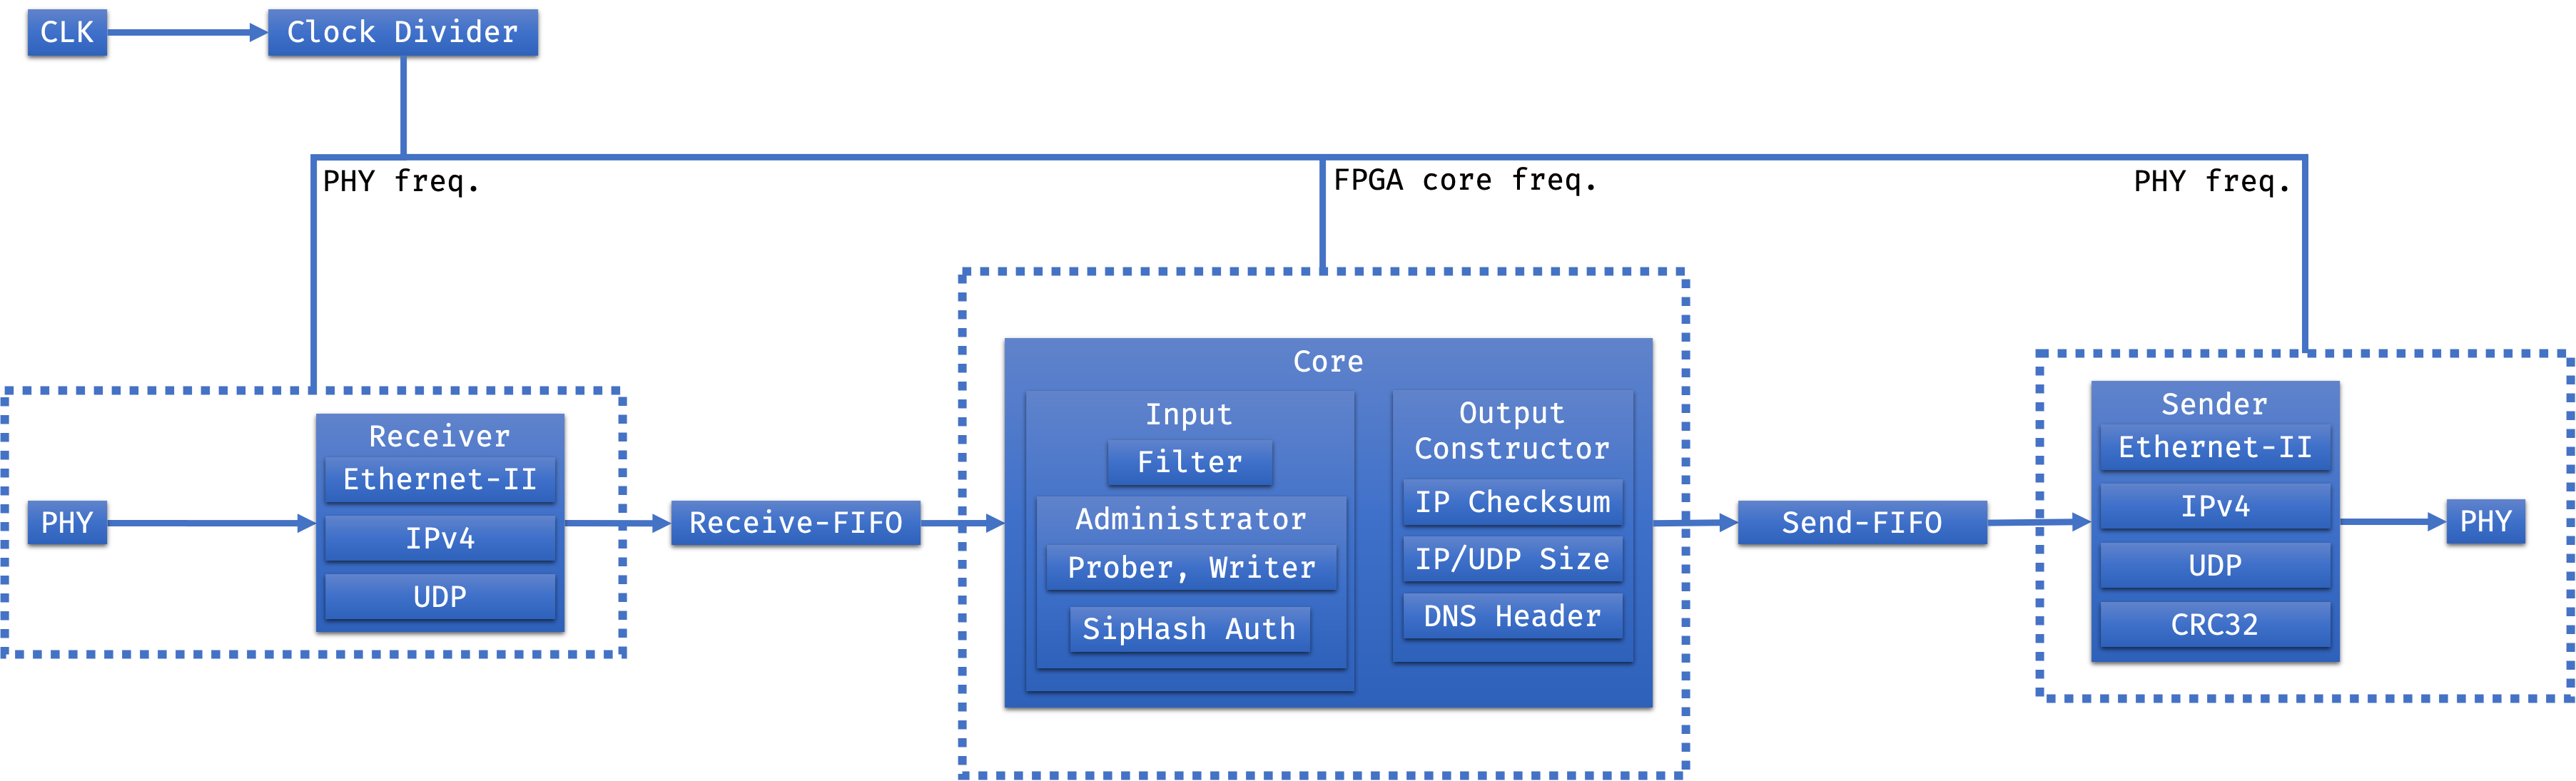
\includegraphics[width=\textwidth]{imgs/hardware-design.png}
  \caption{Hardware Architectural Design}
\end{figure}

\begin{figure}[h!]
  \makebox[\textwidth][c]{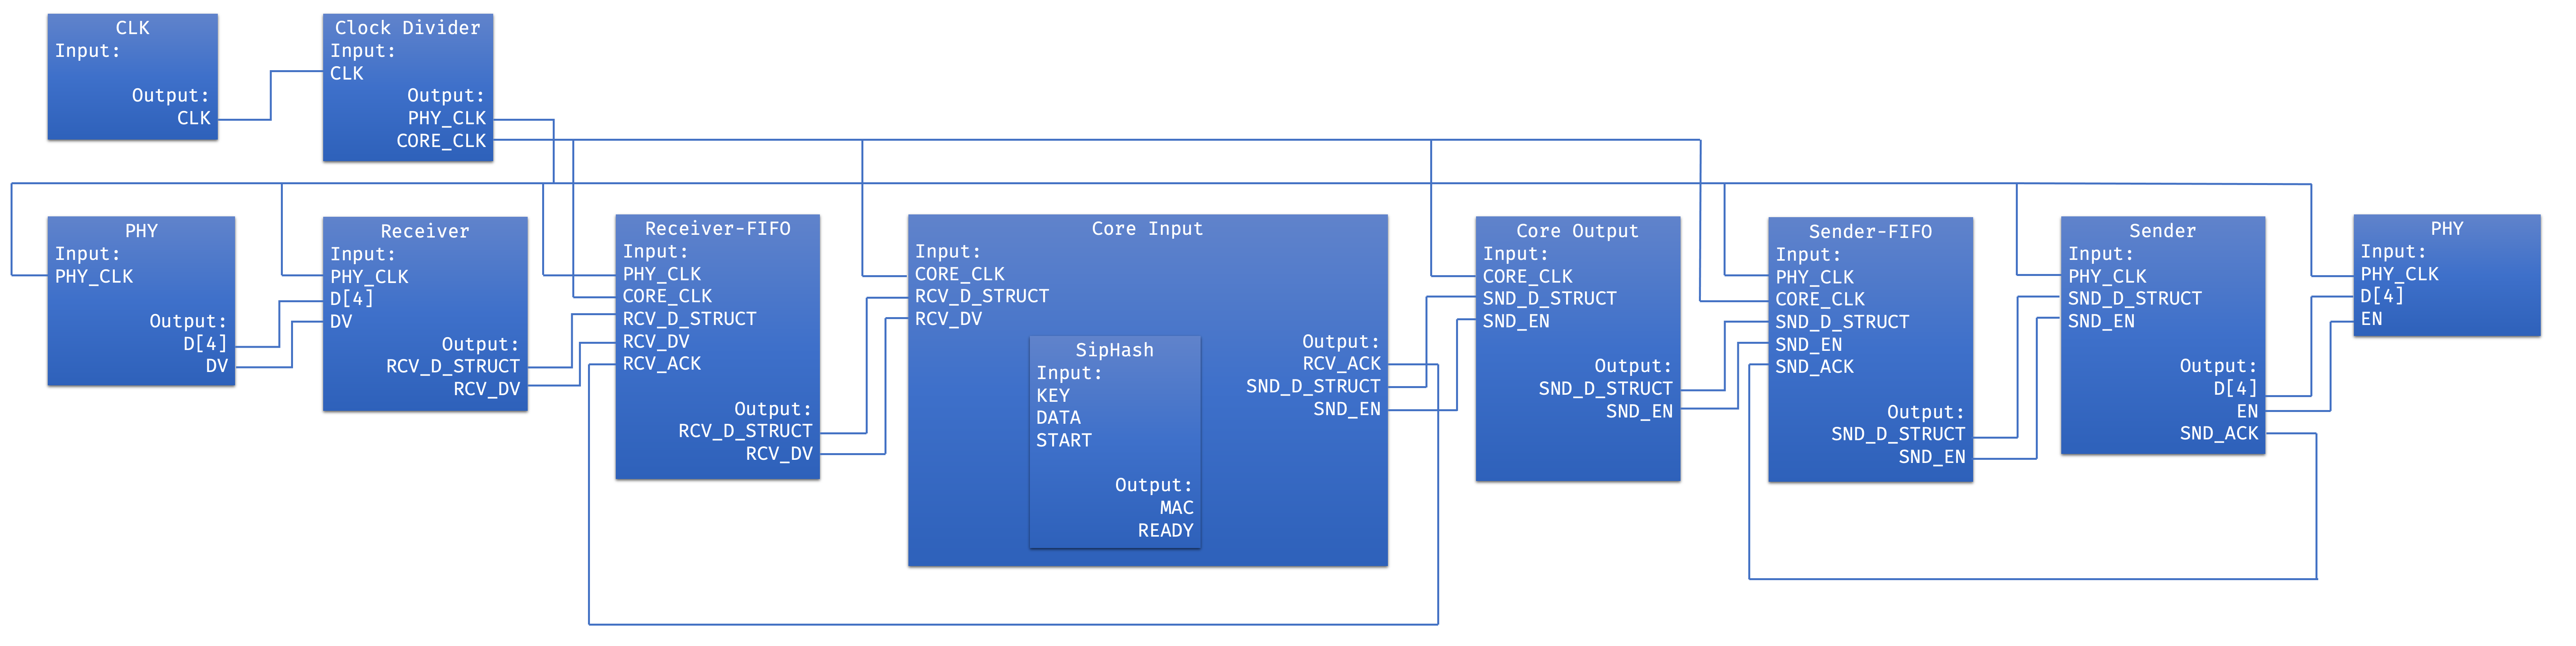
\includegraphics[width=1.2\textwidth]{imgs/hardware-signal.png}}
  \caption{Hardware Signal Design}
\end{figure}

\begin{figure}[h!]
  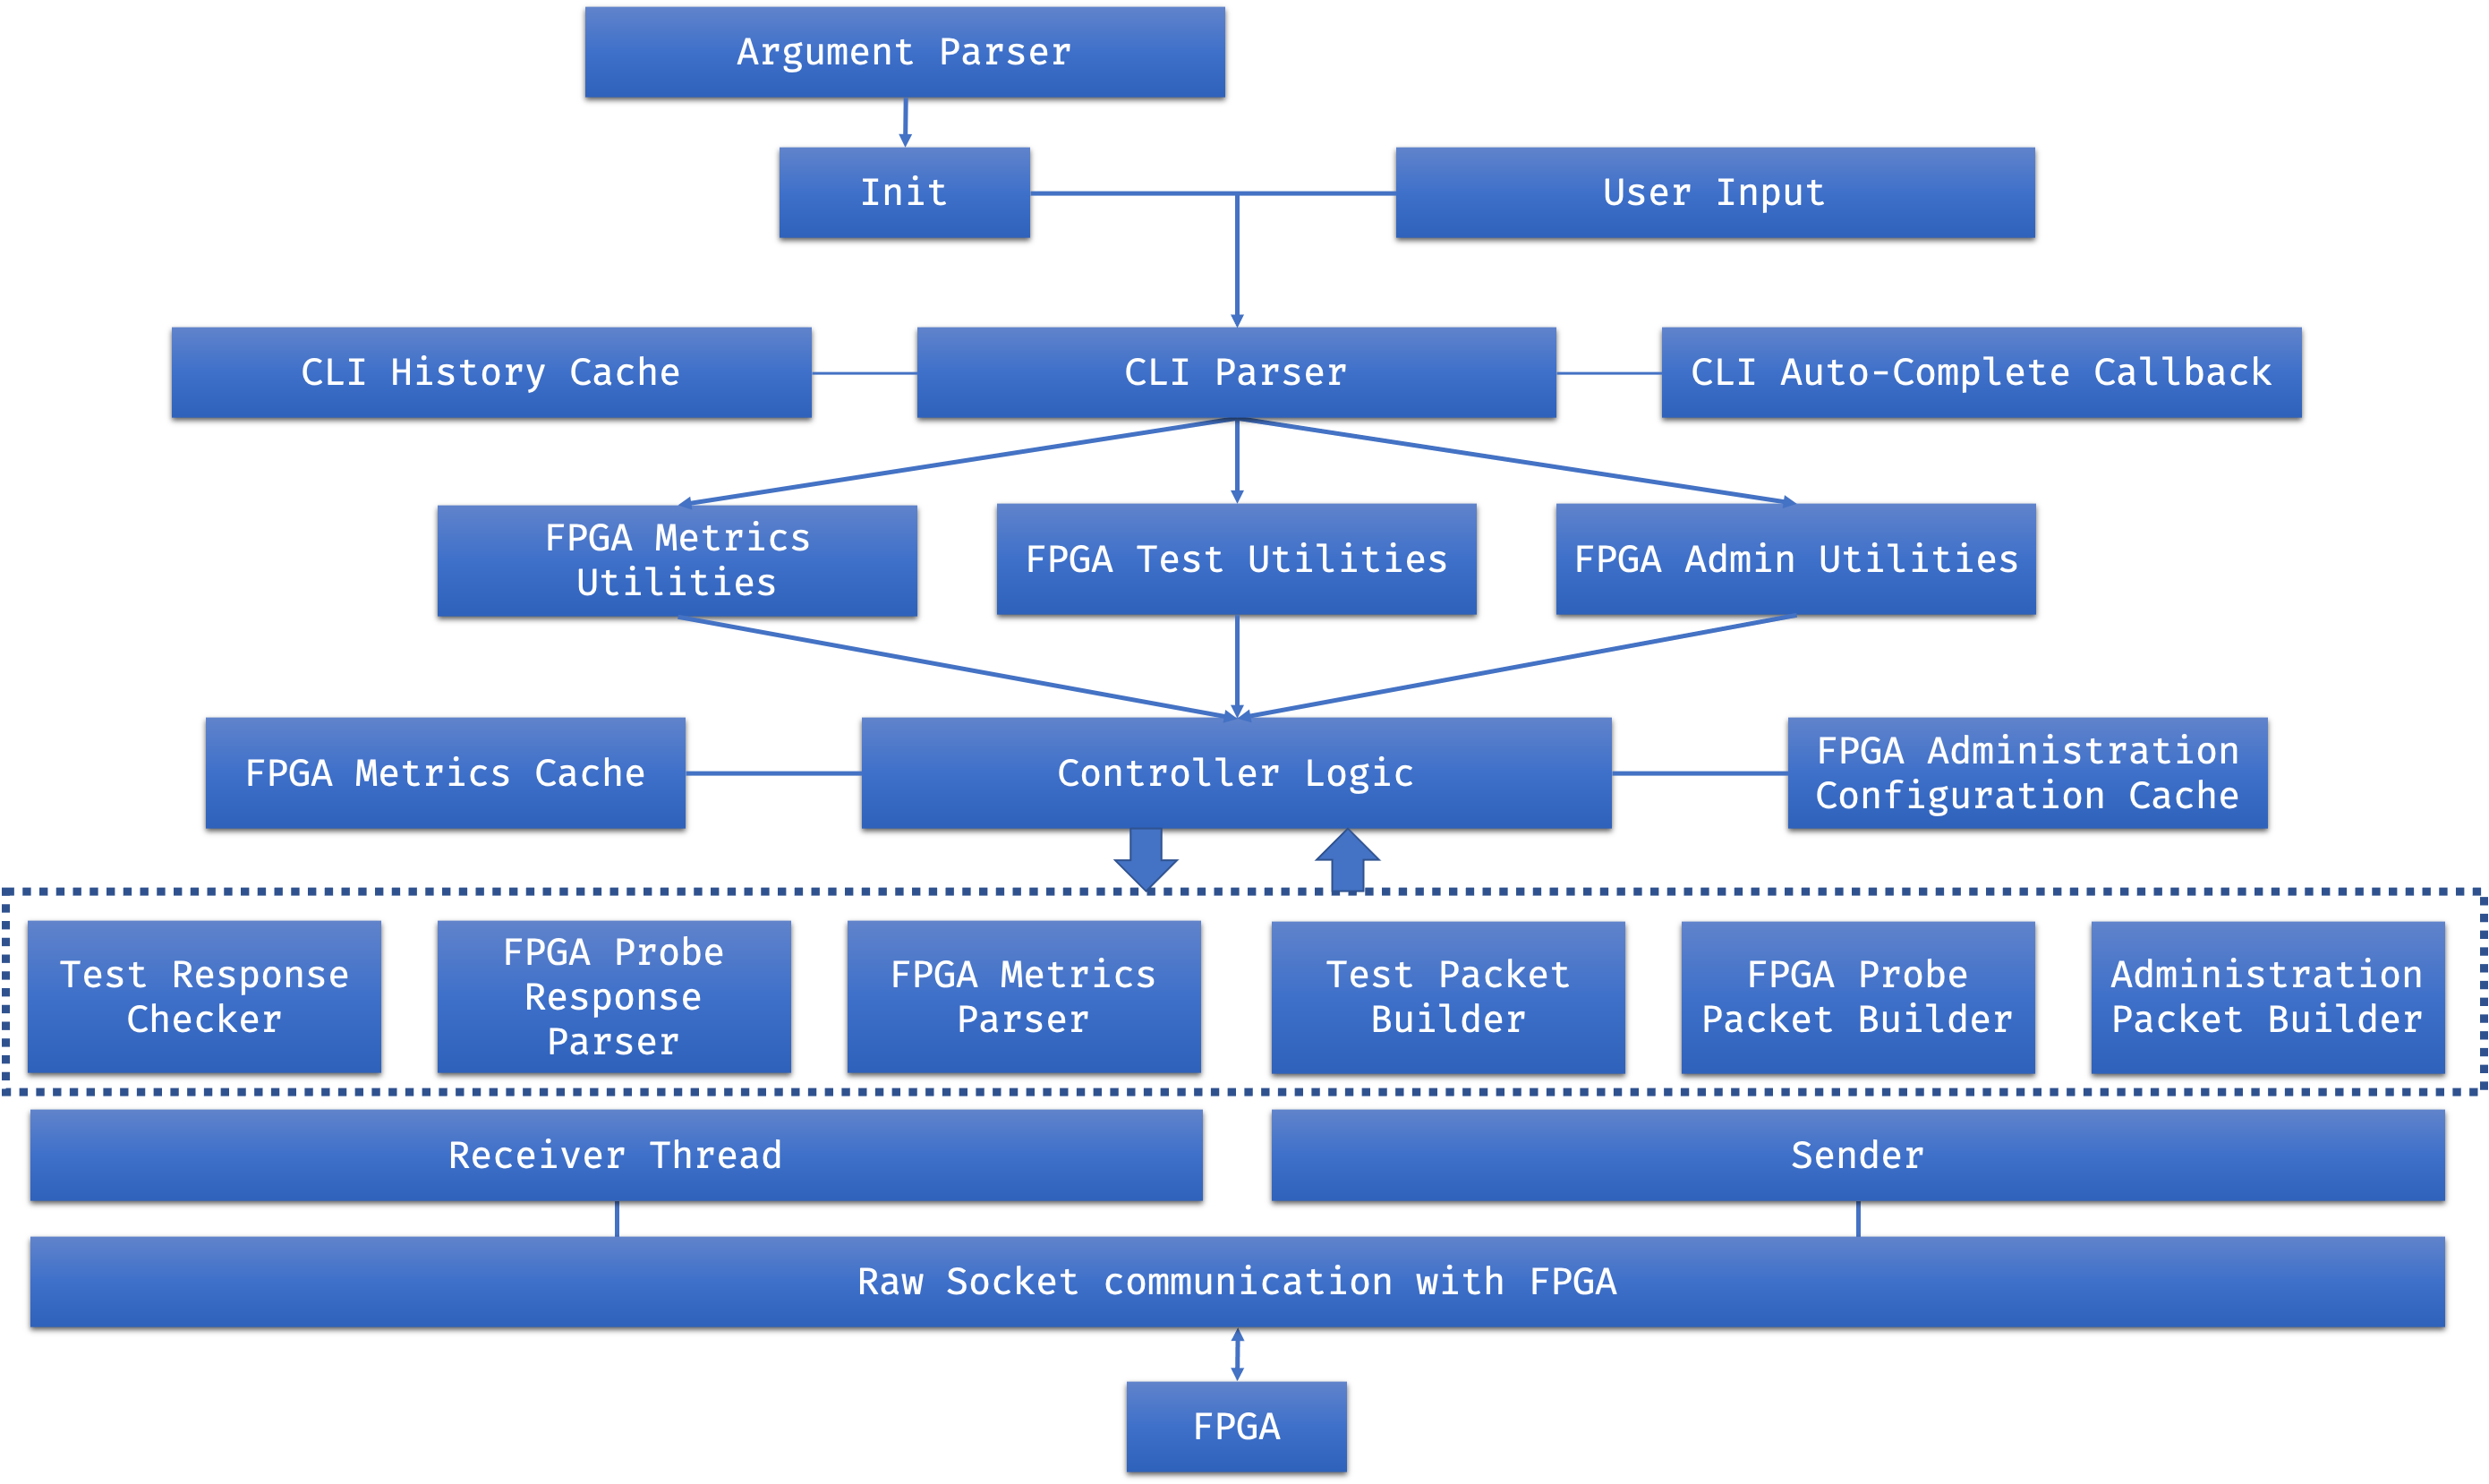
\includegraphics[width=\textwidth]{imgs/software-design.png}
  \caption{Software Design}
\end{figure}

\section{System Usage Sample Topology}

\begin{figure}[h!]
  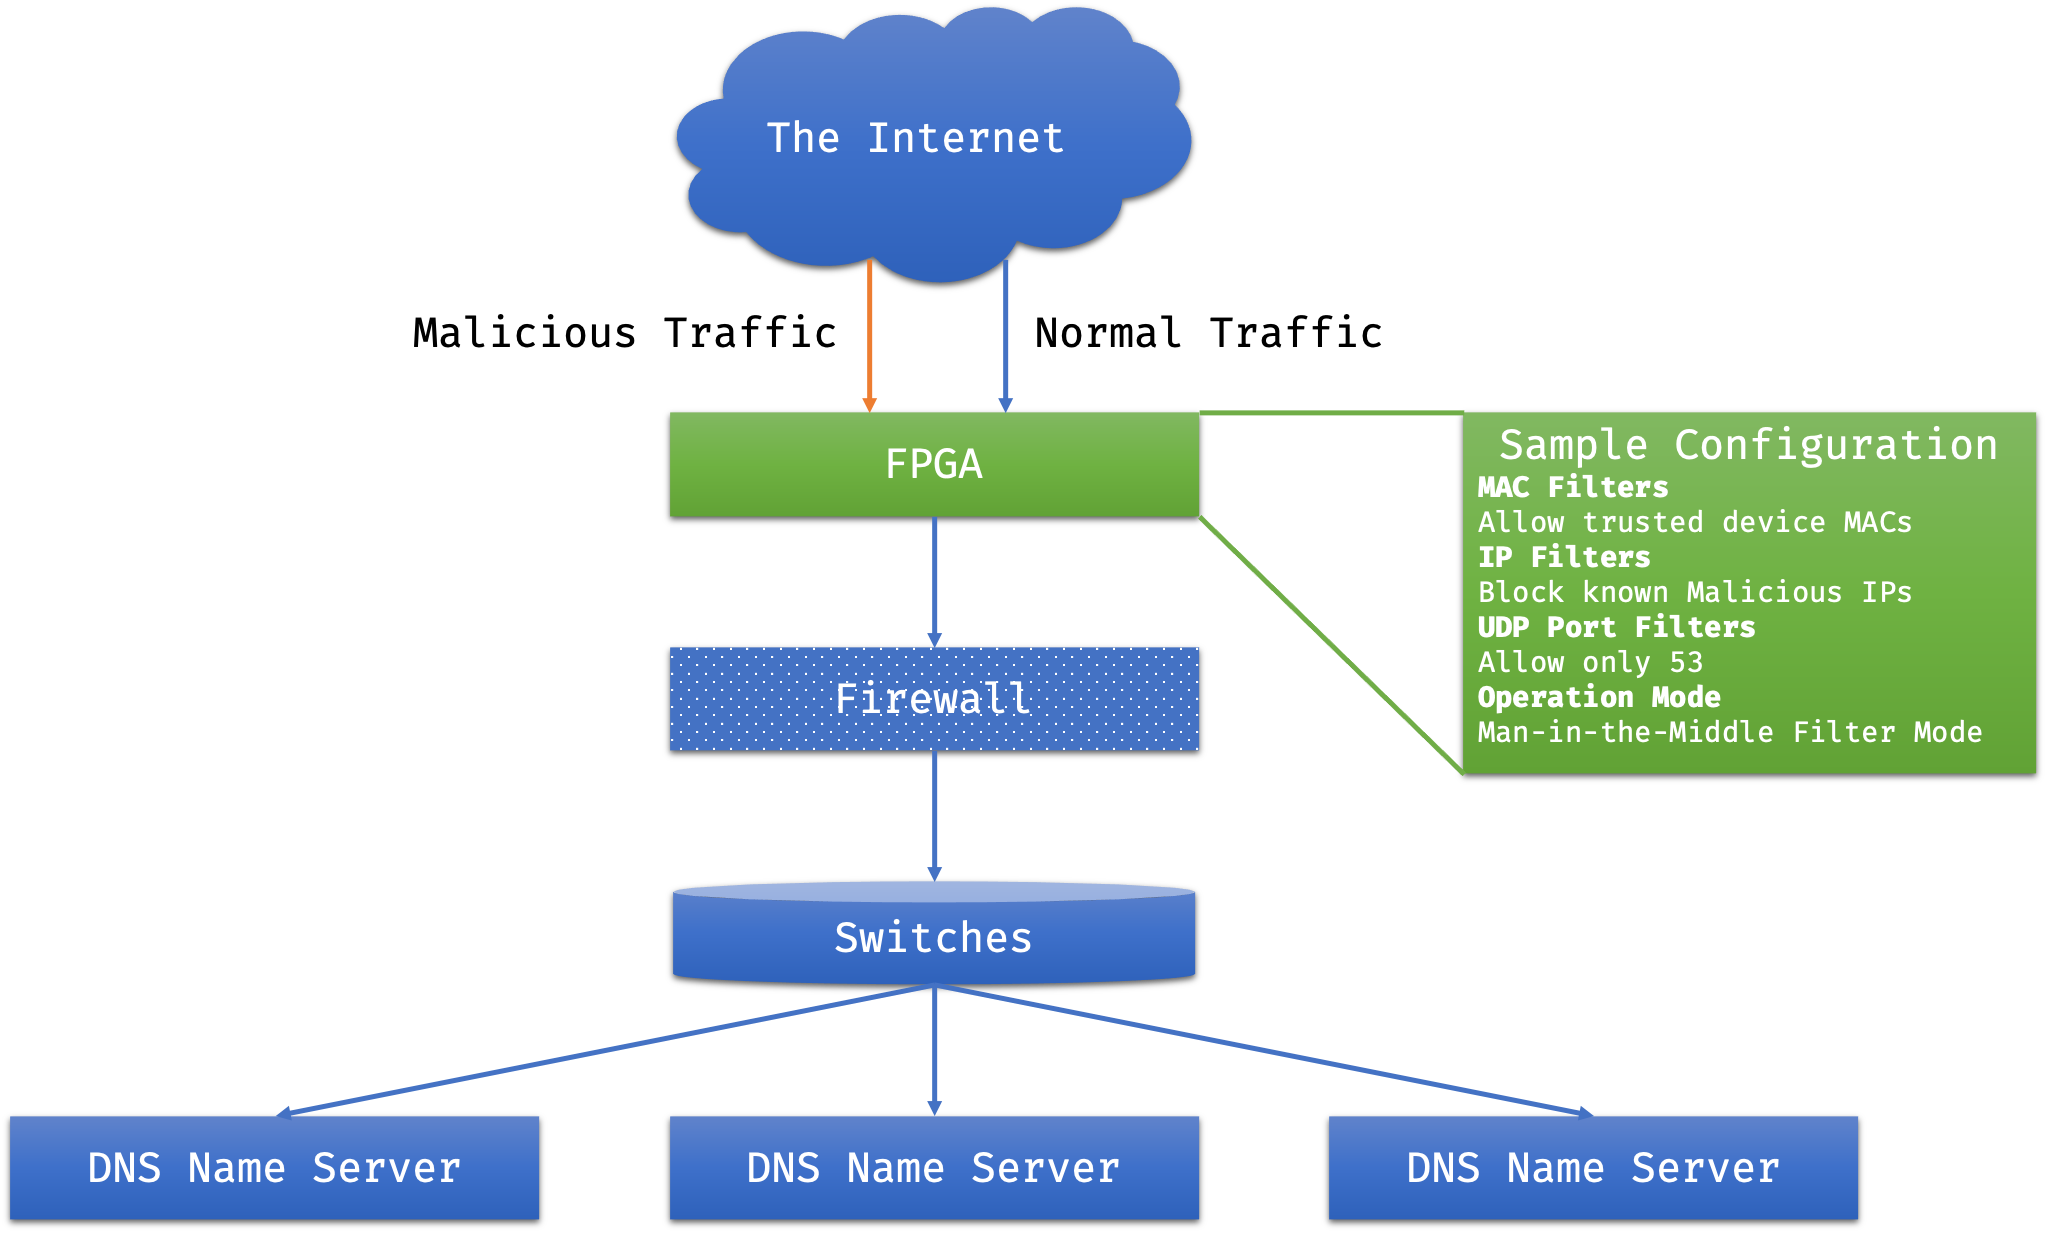
\includegraphics[width=\textwidth]{imgs/man-in-the-middle-topology.png}
  \caption{Man-in-the-Middle FPGA sample topology}
\end{figure}

\begin{figure}[h!]
  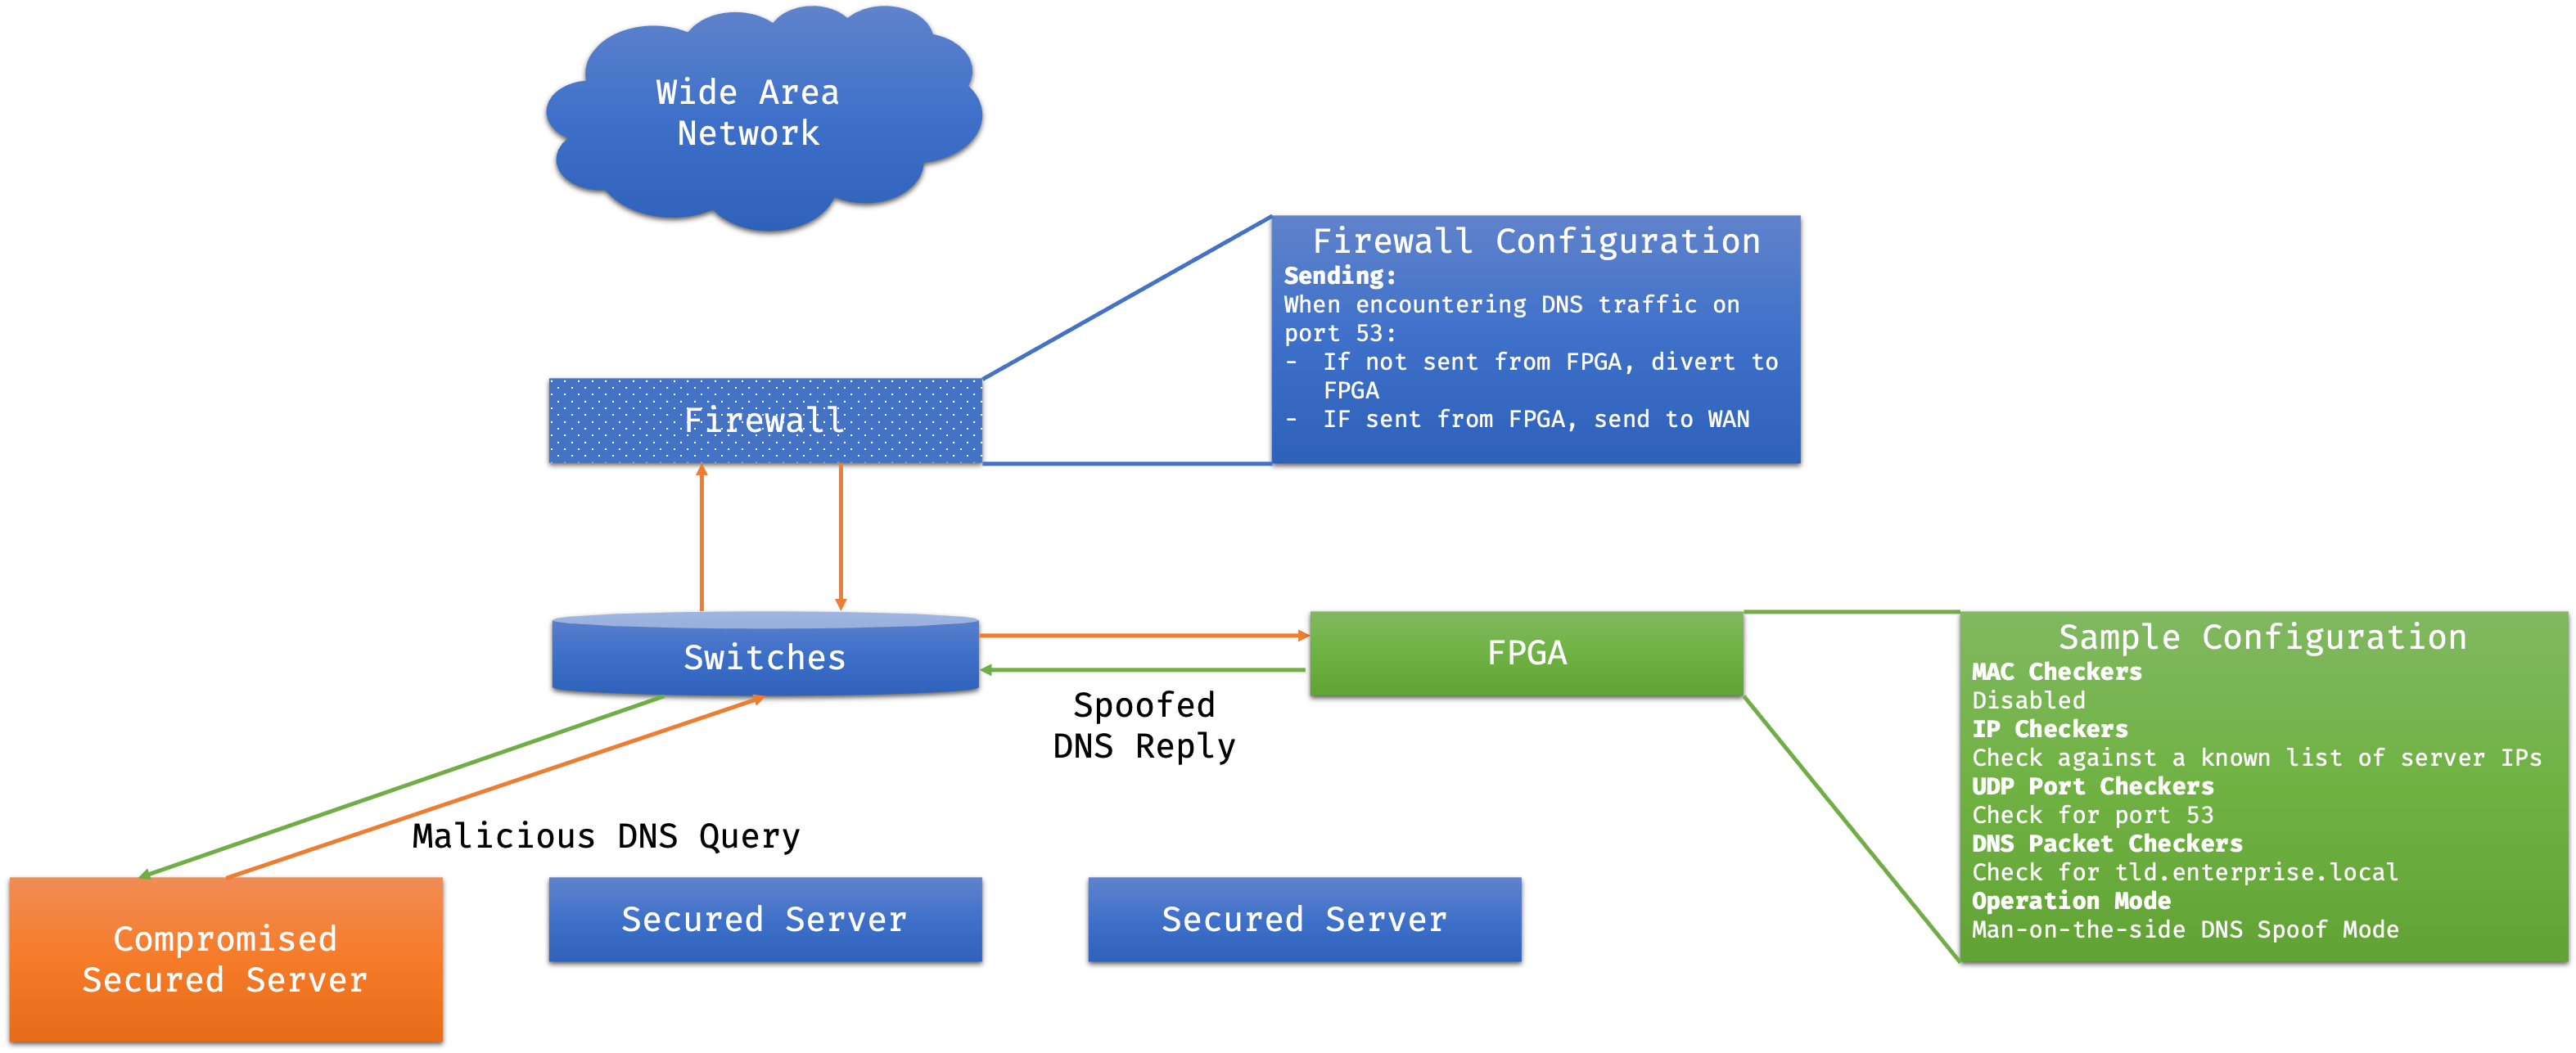
\includegraphics[width=\textwidth]{imgs/man-on-the-side-malicious-dns-query.png}
  \caption{Man-in-the-Middle FPGA sample topology}
\end{figure}

\begin{figure}[h!]
  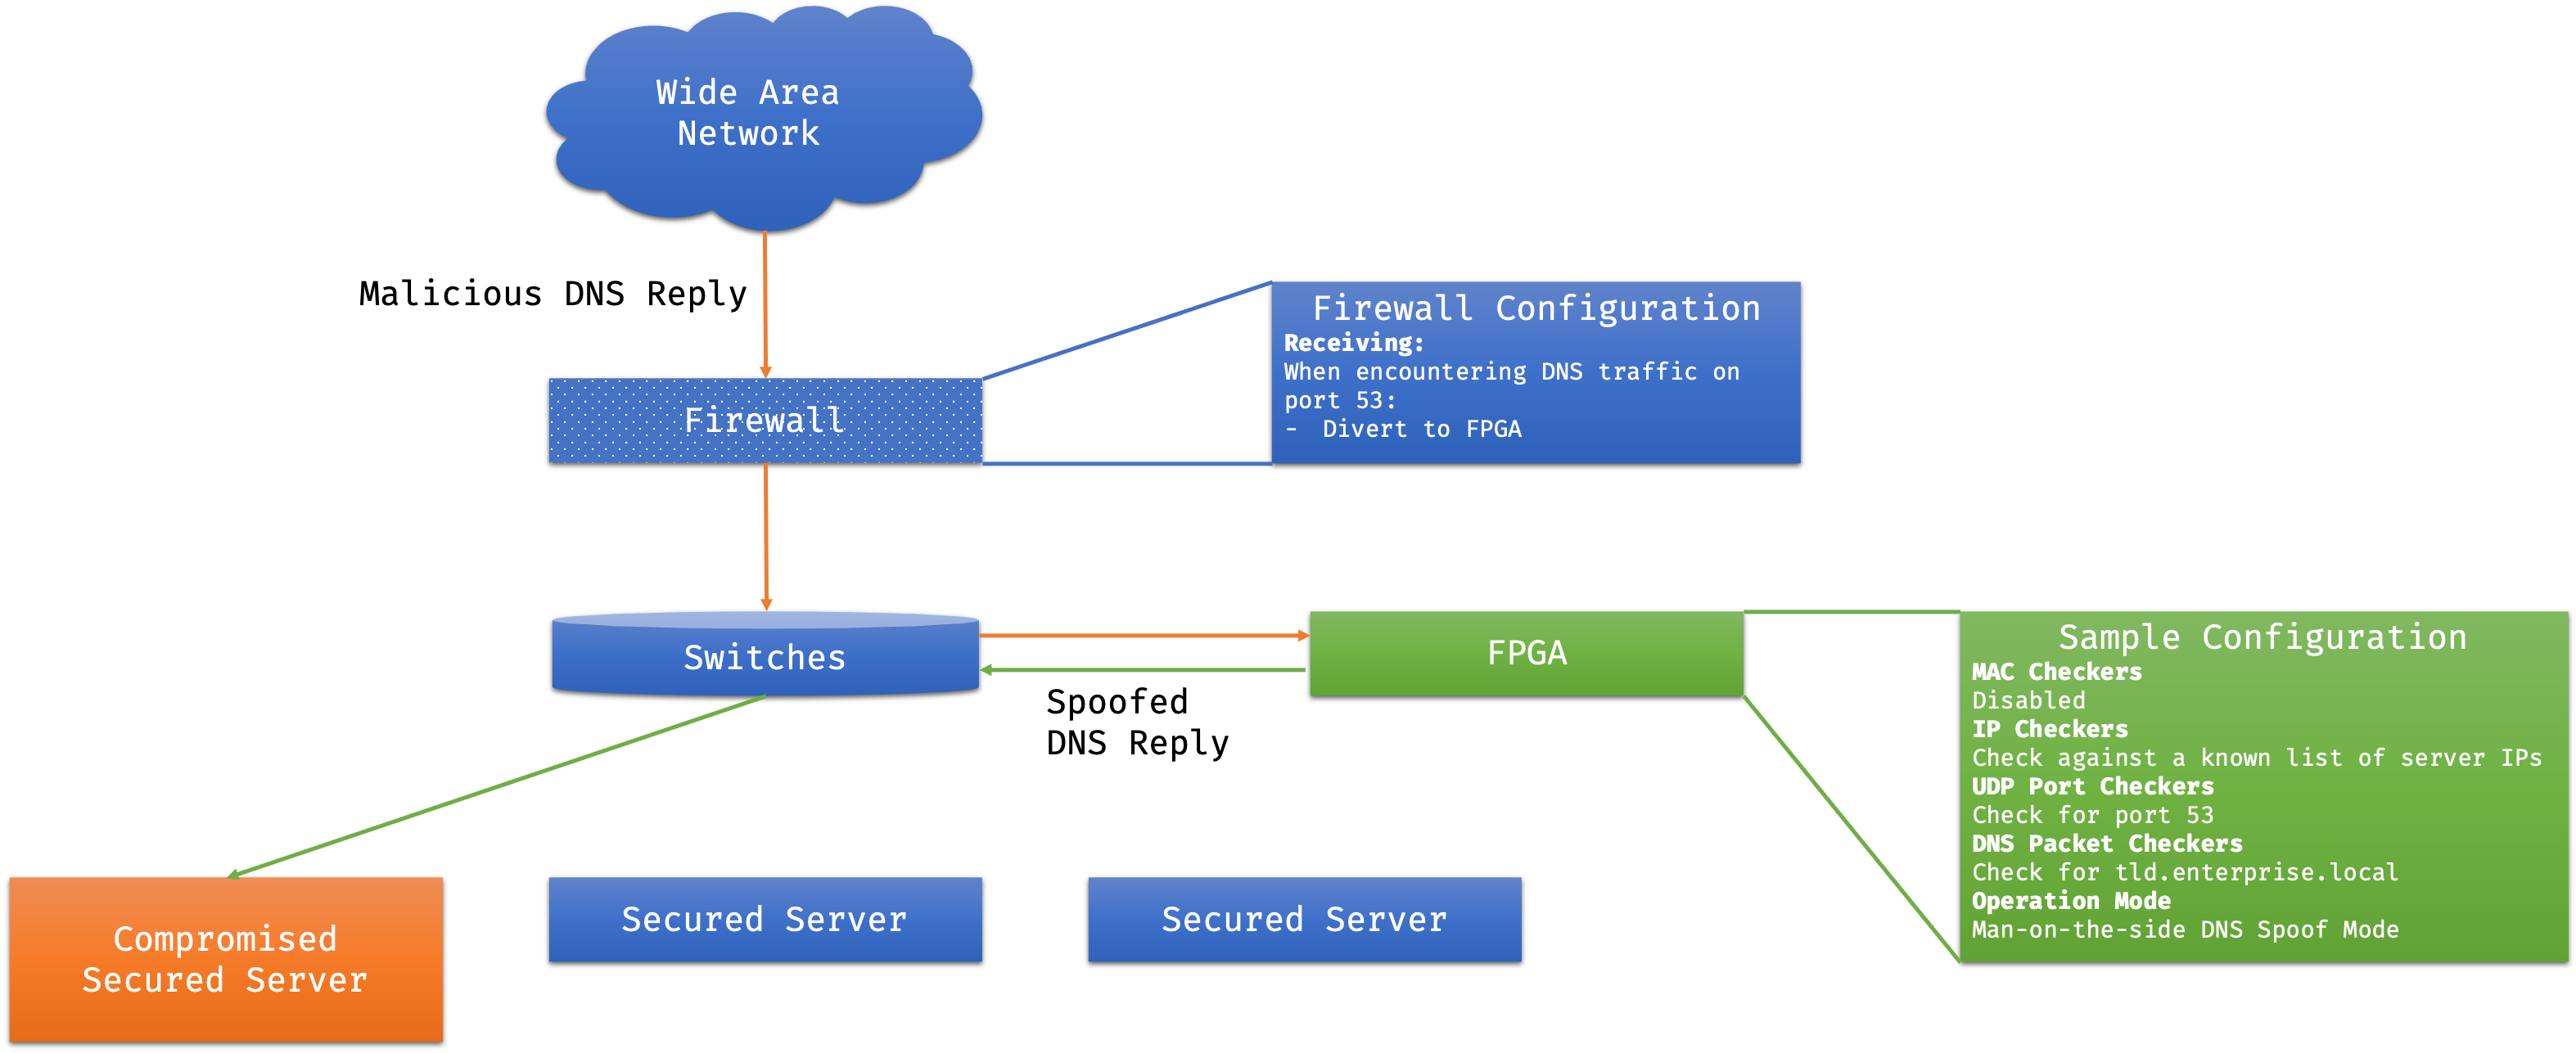
\includegraphics[width=\textwidth]{imgs/man-on-the-side-malicious-dns-reply.png}
  \caption{Man-in-the-Middle FPGA sample topology}
\end{figure}

\begin{figure}[h!]
  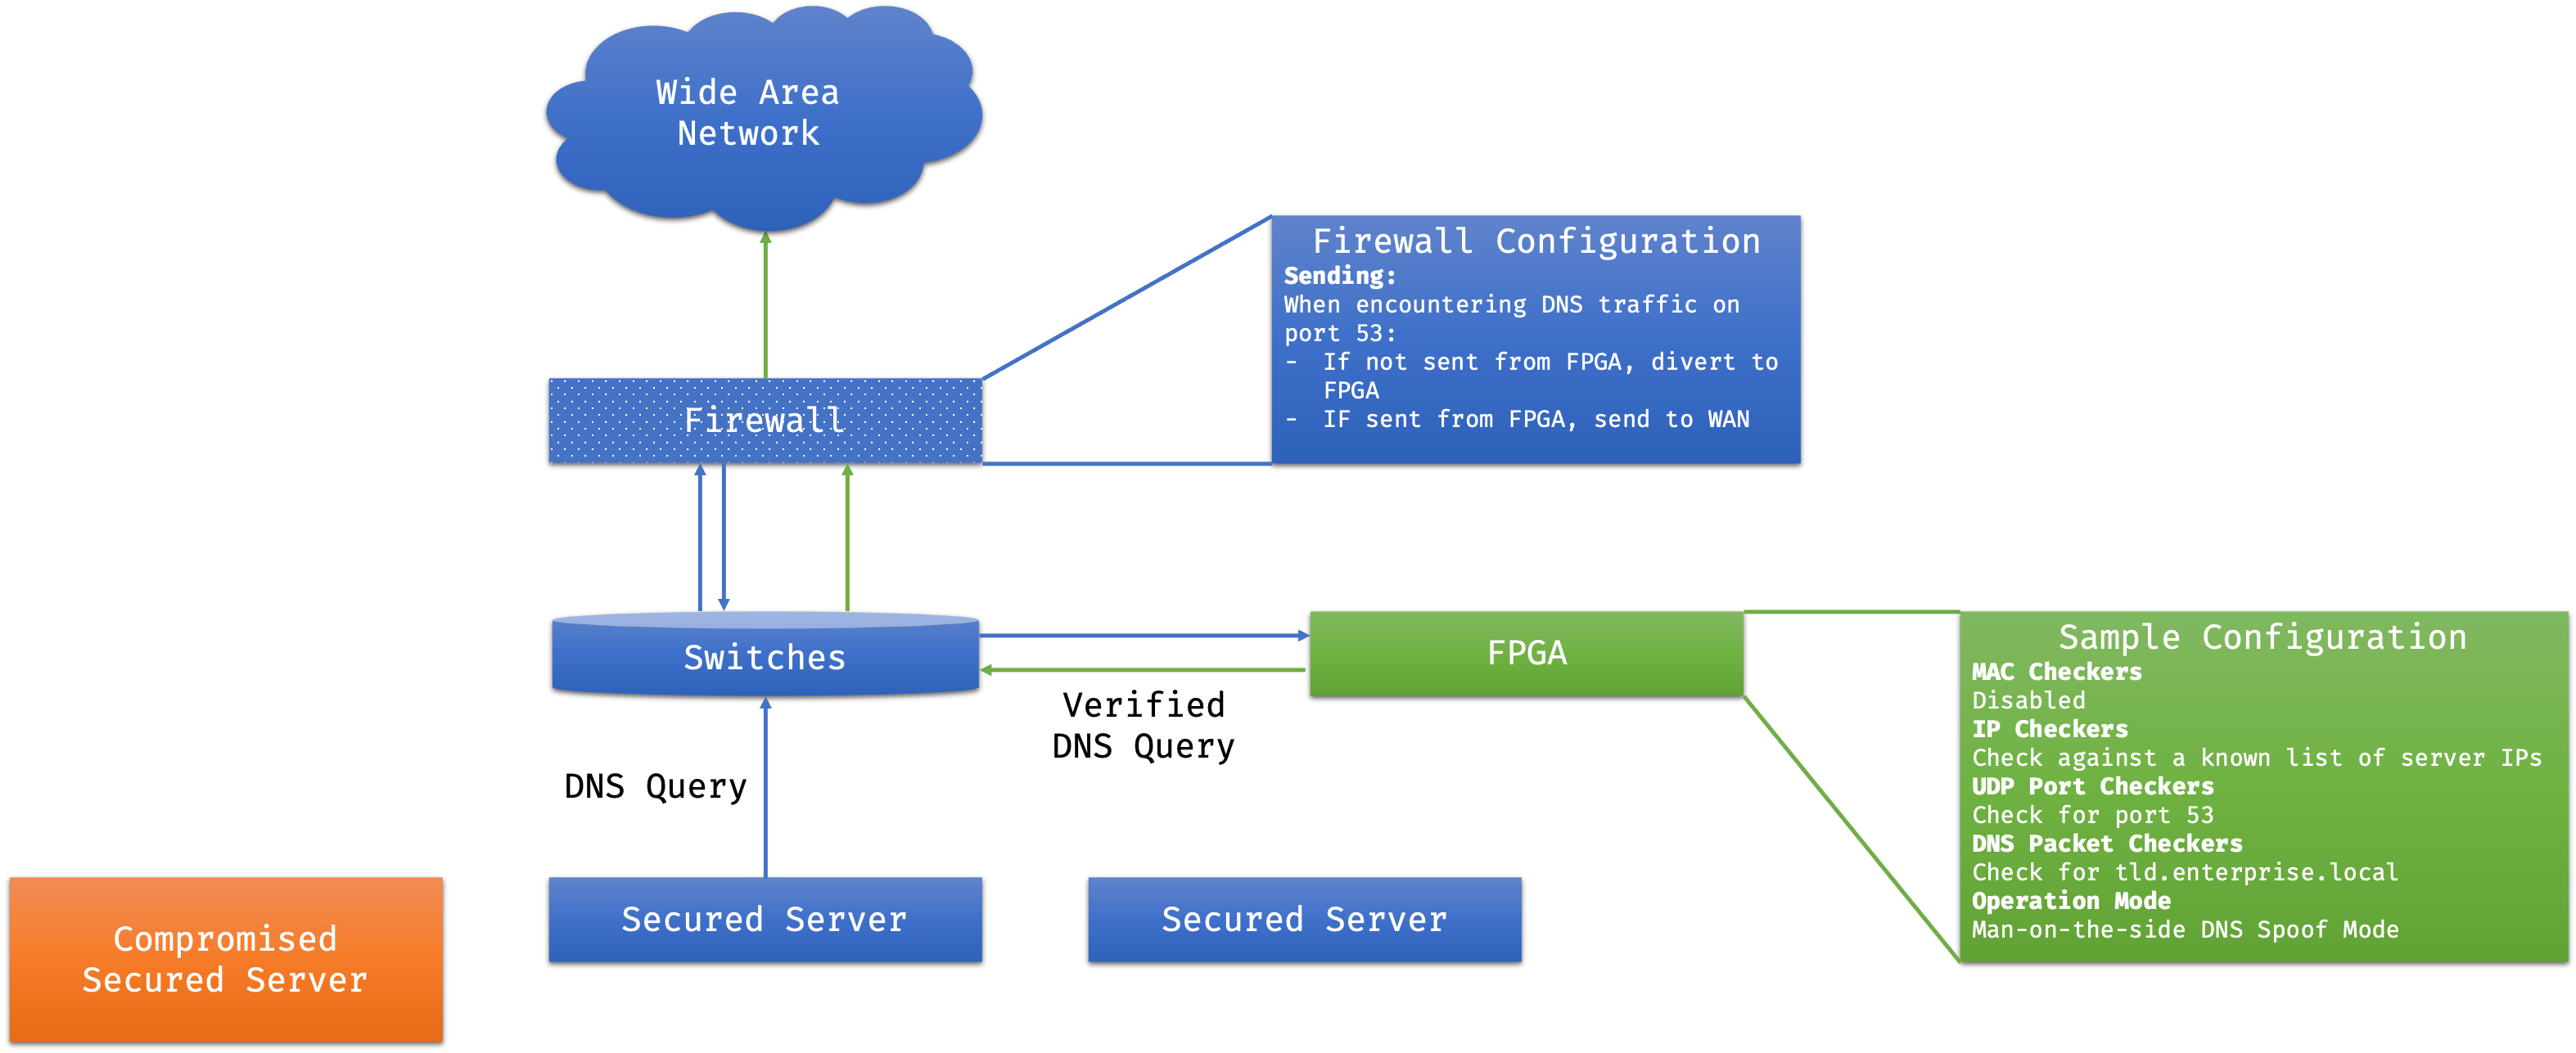
\includegraphics[width=\textwidth]{imgs/man-on-the-side-valid-dns-query.png}
  \caption{Man-in-the-Middle FPGA sample topology}
\end{figure}

\begin{figure}[h!]
  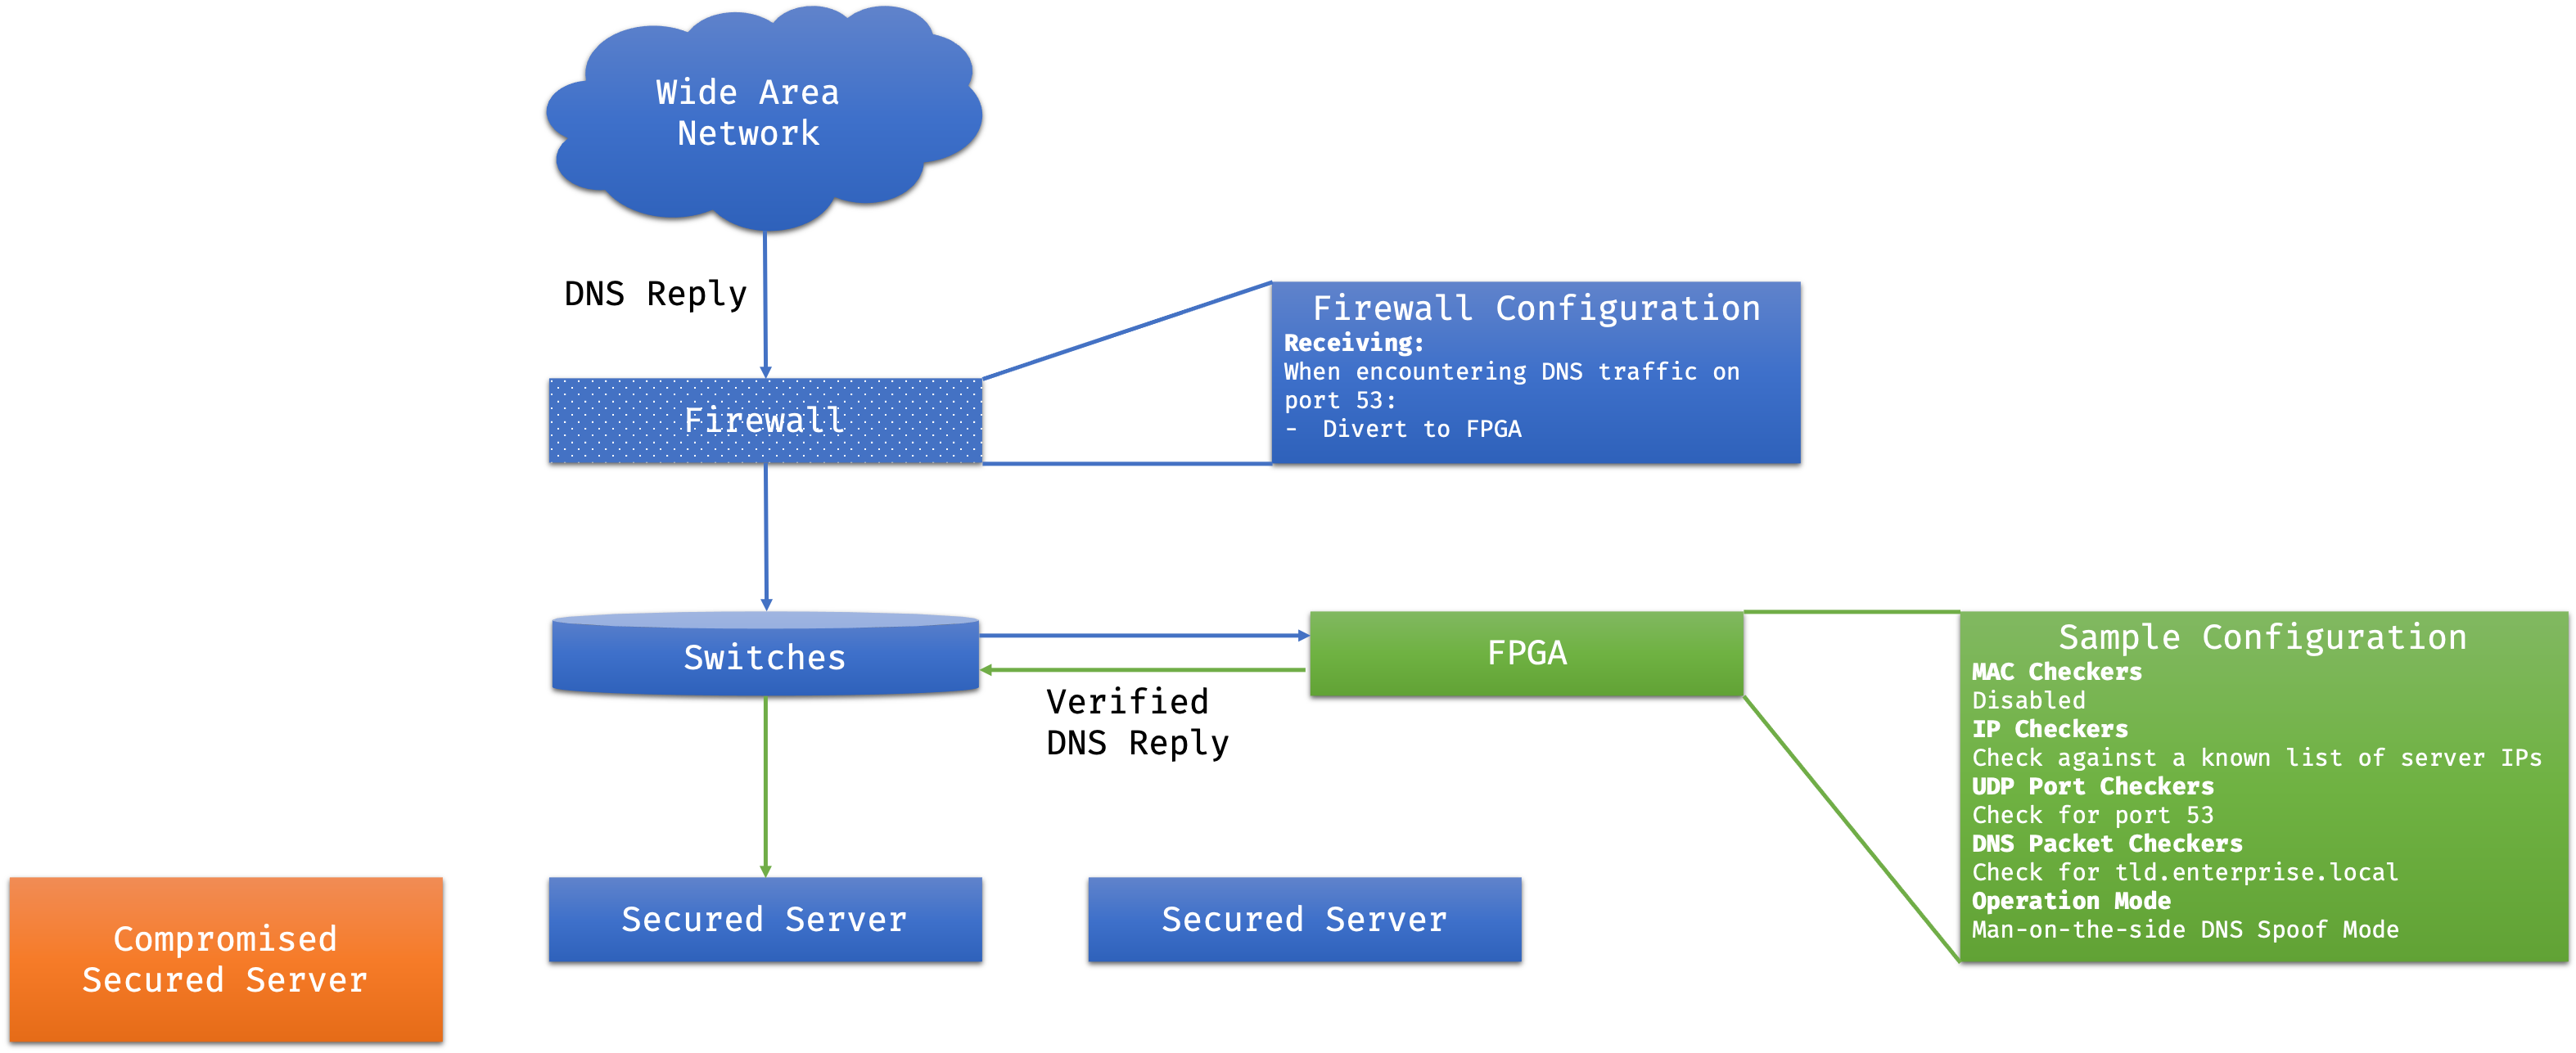
\includegraphics[width=\textwidth]{imgs/man-on-the-side-valid-dns-reply.png}
  \caption{Man-in-the-Middle FPGA sample topology}
\end{figure}


\chapter{Implementation}

\section{Hardware Implementation}

\section{Hardware Debugging}

\section{Software Control System}

\chapter{Validation and Evaluation}

\section{Simulation Unit Test-bench}

\section{Hardware Software Integration}

\section{Performance Evaluation}

\chapter{Conclusions and Future Work}

\section{Conclusions}

\section{Future Work}
How the project might be continued, but don't give the impression you ran out of time!

\addcontentsline{toc}{chapter}{References}
\printbibliography[title=References]

\appendix

\chapter{Project Demo}

\chapter{Code Listing}

URL \url{https://github.com/magetron/cpu-fpga-nwofle}

\chapter{Original Project Proposal}

\end{document}